При анализе технических решений целесообразно уделить внимание разработкам компаний, 
которые занимают лидирующие позиции в данной области. Одной из таких компаний является "Tesla Inc". 
Далее будет приведено устройство батареи, широко известной модели "Tesla Model S".



\begin{figure}[h]
    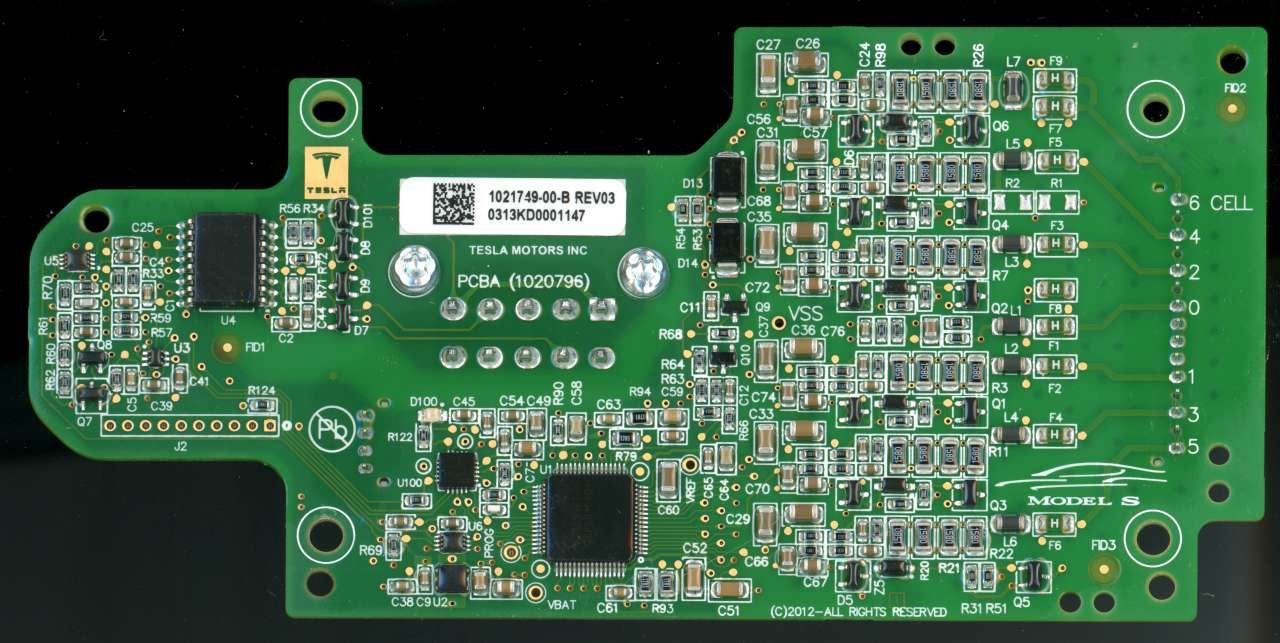
\includegraphics[width=\linewidth]{img/tesla_bms.jpg}
    \caption{BMS модуля батареи Tesla S}
    \label{fig:tesla_bms}
\end{figure}
% Figure \ref{fig:boat1} shows a boat.

% \begin{figure}[h]
% 	\centering
% 	\begin{minipage}{0.45\linewidth}
% 		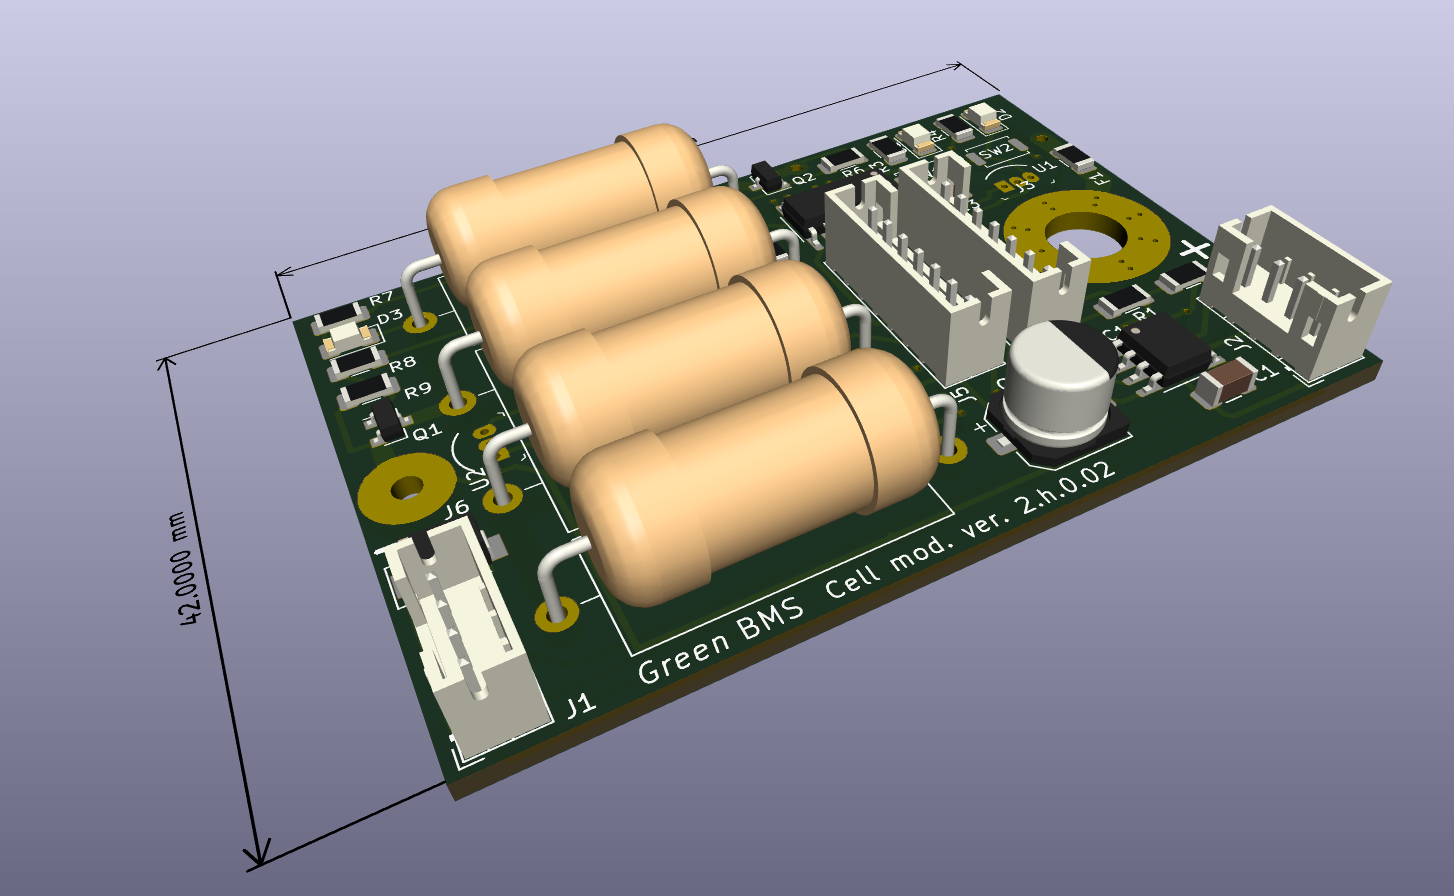
\includegraphics[width=\linewidth]{img/smart_bms_cell_1.png}
% 		\subcaption{Плата-slave(вид сбоку)}
% 		% \label{fig:smart_bms_slave_1}
% 	\end{minipage}
% 	\begin{minipage}{0.45\linewidth}
% 	    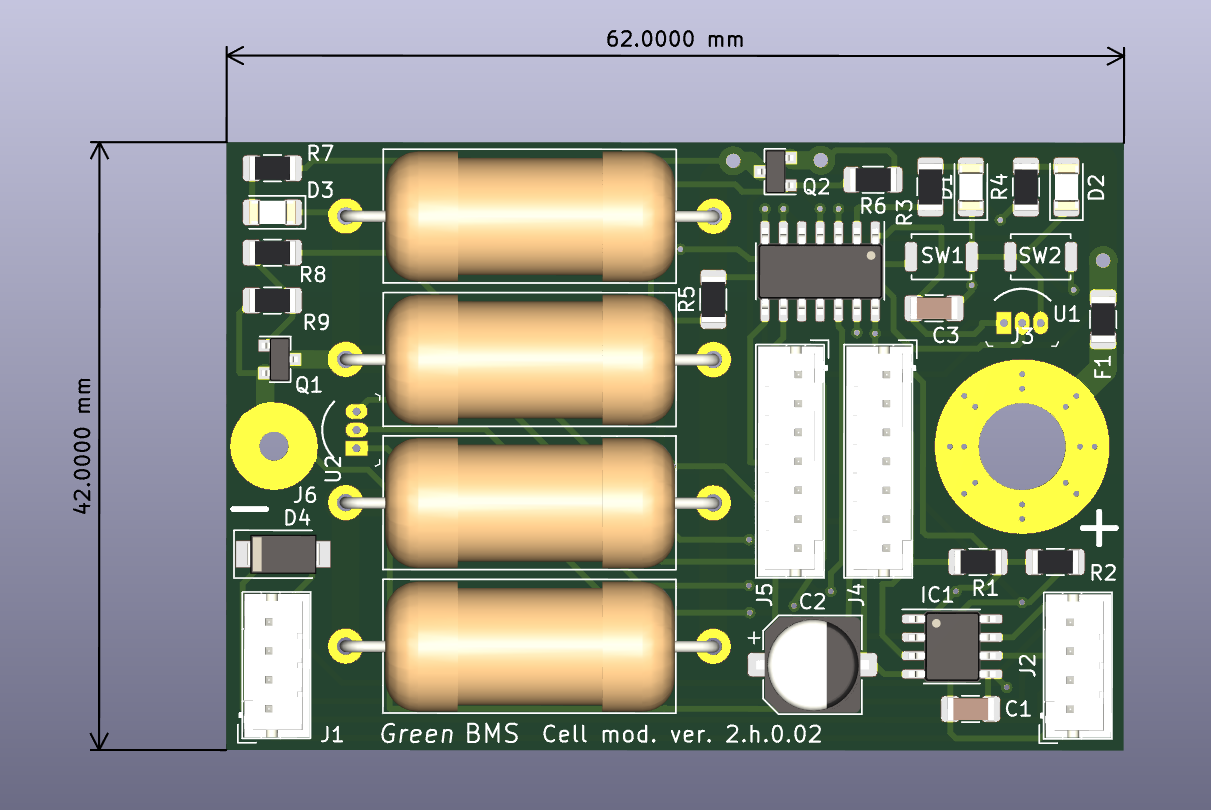
\includegraphics[width=\linewidth]{img/smart_bms_cell_2.png}
% 	    \subcaption{Плата-slave(вид сверху)}
% 	    % \label{fig:smart_bms_slave_2}
%         \end{minipage} \\	
% 	\begin{minipage}{0.45\linewidth}
% 	    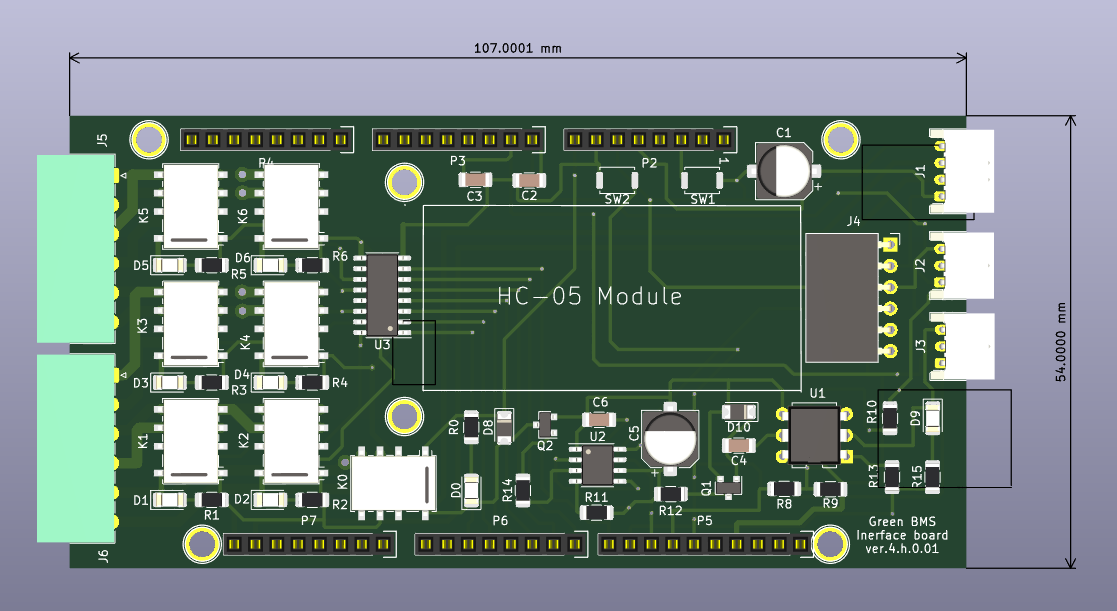
\includegraphics[width=\linewidth]{img/smart_bms_ctrl.png}
% 	    \subcaption{Плата-мастер}
% 	    % \label{fig:smart_bms_master}
%     \end{minipage}
% \caption{Составляющие Smart BMS}
% \label{fig:smart_bms}
% \end{figure}